\documentclass[12pt, a4paper, openany]{report}
\def\VersionRapport{1.0}
\usepackage[utf8]{inputenc} % un package
\usepackage[T1]{fontenc}      % un second package
\usepackage[francais]{babel}  % un troisième package
\usepackage{layout}
\usepackage[top=2.7cm, bottom=2.5cm, left=3.5cm, right=3cm]{geometry}
\usepackage{setspace}
\frenchbsetup{StandardLists=true} % à inclure si on utilise \usepackage[french]{babel}
%\usepackage{enumitem}
\usepackage[shortlabels]{enumitem}
\usepackage{amssymb}
\usepackage{color}
\usepackage{listings}
\definecolor{dkgreen}{rgb}{0,0.6,0}
\definecolor{gray}{rgb}{0.5,0.5,0.5}
\definecolor{mauve}{rgb}{0.58,0,0.82}
\definecolor{rougecerise}{rgb}{0.73,0.043,0.043}
\lstset{frame=tb,
  language=Matlab,
  aboveskip=3mm,
  belowskip=3mm,
  showstringspaces=false,
  columns=flexible,
  basicstyle={\small\ttfamily},
  keywordstyle=\color{blue},
  commentstyle=\color{dkgreen},
  stringstyle=\color{mauve},
  breaklines=true,
  breakatwhitespace=true,
  tabsize=3,
  breaklines=true,
  morekeywords={matlab2tikz},
  morekeywords=[2]{1}, 
  keywordstyle=[2]{\color{black}},
  identifierstyle=\color{black},
  numbers=left,
  numberstyle={\tiny \color{black}},
  numbersep=9pt, 
  emph=[1]{for,end,break},
  emphstyle=[1]\color{red}
}
\usepackage{multirow} % pour les tableaux
\usepackage[table]{xcolor} % pour les tableaux
\usepackage{verbatim}
%\usepackage{subcaption}
\usepackage{graphicx}
\usepackage{moreverb}
\usepackage{url}
\usepackage{pst-all}
\usepackage{eso-pic,graphicx}
\usepackage{caption} 
\usepackage[colorlinks=true,urlcolor=blue,linkcolor=red]{hyperref}
\usepackage{array}
\usepackage[toc,page]{appendix}
\usepackage[off]{auto-pst-pdf}
\usepackage{hyperref} % pour le sommaire table des matières
\AddThinSpaceBeforeFootnotes % à insérer si on utilise \usepackage[french]{babel}
\FrenchFootnotes % à insérer si on utilise \usepackage[french]{babel}
\usepackage{fancyhdr}
\pagestyle{headings}
\usepackage{pifont}  %pour les puces
\usepackage{amsmath,amsfonts,amssymb} %pour les puces
\usepackage{subfig}
\usepackage{verbatim} % pour le code en annexe 
%%%%%%%colones 
\newcolumntype{R}[1]{>{\raggedleft\arraybackslash }b{#1}}
\newcolumntype{L}[1]{>{\raggedright\arraybackslash }b{#1}}
\newcolumntype{C}[1]{>{\centering\arraybackslash }b{#1}}
%%%%%%% 
\renewcommand{\appendixpagename}{Annexes}
\renewcommand{\appendixtocname}{Annexes}
\title{Theme: Compte Rendu Représentation et Analyse des Systèmes Non Linéaires}
\author{NAIMI \bsc{Nabil} \\ KHERBICHE \bsc{Ali}}
\date{2018-2019}
%new
\newcommand{\HRule}{\rule{\linewidth}{0.5mm}}

\begin{document}

%\selectlanguage{francais}
\pagenumbering{arabic} 
\makeatletter
\begin{titlepage}
\begin{sffamily}
\begin{center}
    % Upper part of the page. The '~' is needed because \\
    % only works if a paragraph has started.
    
\includegraphics[scale=0.5]{Logo_UT3.jpg}~\\[1cm]
    \textsc{\LARGE M1 ISTR-RODECO  }\\[1cm]
    \textsc{\Large Compte Rendu Représentation et Analyse des Systèmes Non Linéaires}\\[1cm]
    % Title
    \HRule \\[0.4cm] % saut de ligne
    { \huge  \textsc {Analyse de stabilité d'un système à bac d'eau \\[0.4cm] }}

    \HRule \\[1cm]   % sous de ligne 
    
\includegraphics[scale=0.1]{logomaster.jpg}
    \\[1cm]
    % Author and supervisor
    \begin{minipage}{0.4\textwidth}
      \begin{flushleft} \large
         \textsc{\emph {Fait par:} \\KHERBICHE Ali\\ NAIMI Nabil}  
          \newline
          Promotion 2018-2019 \\
      \end{flushleft}
    \end{minipage}
    \begin{minipage}{0.4\textwidth}
      \begin{flushright} \large
        %%\emph{Tuteur et}
        \emph{Tuteur:} \textsc{M Frédéric GOUAISBAUT}
      \end{flushright}
    \end{minipage}
    \vfill
    % Bottom of the page
    {\large Avril 2018}
  \end{center}
  \end{sffamily}                
  \end{titlepage}  
\makeatother
   
%*********************** somaire **************
\renewcommand{\contentsname}{Sommaire}
\tableofcontents
%*********************** listes des figures **************
\listoffigures
%*********************** listes des tableaux **************
%\listoftables

\chapter*{\textsc{Introduction}}
\addcontentsline{toc}{chapter}{\textsc{Introduction}}

	\paragraph{} On souhaite évaluer le comportement dynamique d’un dispositif de régulation de niveau. Dans un premier temps on étudie un système composé par un seul bac d’eau, une entrée et une fuite et ensuite on étudie un
système composé par deux bacs d’eau communiquants entre eux sans/avec entrée et fuite.
\chapter{\textsc{Analyse du procédé un bac d'eau}}
\section{\textsc{Le procédé}}
 
 	\paragraph{} Le système représenté sur la Figure 1 est composé d’un bac cylindrique de section $S$. Il se vide par un cylindre de section $S_n << S$. Une pompe de débit constant $Q_0$ permet de remplir le bac. Lors de cette manipulation, nous allons nous intéresser au régime libre du niveau de l’eau $H(t)$.
\par Les valeurs données par le constructeur sont : $Q_0 = 12$x$10^{-5}m^3/s, S = 0.0154m^2$ et $S_n = 5$x$ 10^{-5} m^2$. La valeur initiale est $H(0) = 0m$.
\par On suppose que la vitesse de $H(t), v(t),$ est plus petite que la vitesse du fluide qui sort par le cylindre de
section $S_n , v_n (t),$ c.à.d. $v(t) << v_n (t)$. De même, on suppose que le diamètre du cylindre de section $S_n$ soit négligeable devant la hauteur $H(t)$.
	
	\begin{center}
	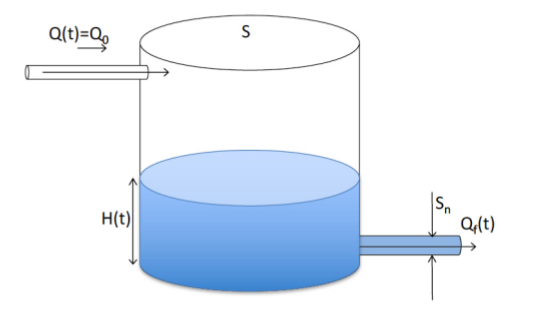
\includegraphics[scale=0.5]{1bac.png}
	\captionof{figure}{\textit{Un bac d'eau avec source et fuite\\}}
	\label{fig1} 
	\end{center}   

\break

\section{\textsc{Modélisation du système par un bilan de volume }}

\textbf{Hypothèse $1$:} \hspace{2mm} $H(t)>0$\\

Loi de conservation de volume:
\[\text{Variation volume $=$ débit entrant - débit sortant.}\]
\begin{center}

$$\left\{
\begin{array}{l}
    V(t)=S\times H(t)\\
    \dot{V}(t)=S\times \dot{H}(t)=(Q(t)-Q_f(t)).dt

\end{array}
\right\}.$$

\end{center}

Loi de conservation de l'énergie: 

\[\text{Variation énergie} = \text{énergie entrante - énergie sortante}\]

\[\text{Variation énergie} = \text{énergie \textit{\textbf{potentielle}}} -\text{ énergie\textit{\textbf{cinétique}}}\]

\[\textbf{TORRICELLI}\]

\textbf{Hypothèse $2$:} \indent La variation d'énergie est égale à zéro.\\

\[Q(t).dt\times g\times H(t)= \frac{1}{2}\times Q(t).dt \times \left(  \frac{Q_f(t)}{S_n}\right)^2\]
\[Q_f(t)=S_n\sqrt{2\times g \times H(t)}\]

On pose: 

$$\left\{
\begin{array}{l}
    x(t)=H(t)\\
    u(t)=Q(t)

\end{array}
\right\}$$

Nous obtenons: \[\dot{x}=\frac{1}{S}\times u - \frac{S_n}{s}\times \sqrt{2\times g \times x}\]


\section{\textsc{Détemination du point d'équilibre}}

Pour l'entrée $Q_0$.\\

\textbf{u} constant $Q_0$; On cherche \textbf{x} tel que \textbf{x} = Cst = $\textbf{X}_0$.\\

\[ 0=\frac{1}{S} \times Q_0 - \frac{S_n}{S} \times \sqrt{2 \times g \times X_0} \indent \longleftarrow f
\left(X_0,Q_0 \right) \]

\[ X_0 = \frac{1}{2 \times g} \times \frac{Q^2_0}{S^2_n} \]


\section{\textsc{Linéarition du système autour du point d'équilibre Q(t)=$Q_0$}}

$$ \left\{
\begin{array}{l}
    u(t)=U_0+\delta_u(t)\\
    x(t)=X_0+\delta_x(t)
\end{array}
\right\} $$\\[0.25 cm]

\[\dot{x}=f(x,u) \indent \Longrightarrow \indent \dot{\delta_x}=f(X0+\delta_x ,Q_0+\delta_u)\]

Dévelopement limité d'ordre $1$:\\

\[\dot{\delta_x}=f(X_0,Q_0)+\frac{\partial f}{ \partial x}(X_0,Q_0)\delta_x + \frac{\partial f}{\partial u}(X_0,Q_0) \delta_u\]

Sachant que : \indent \indent $f(X_0,Q_0)=0$\\
Alors:

\[\dot{\delta_x}=\begin{bmatrix}\frac{\partial f}{ \partial x }\end{bmatrix}.\delta_x + \begin{bmatrix}\frac{\partial f}{\partial u}\end{bmatrix}.\delta_u\]

Le modèle linéarisé s'écrira donc, comme suite:\\

\[\dot{\delta_x}=\begin{bmatrix}-\frac{S_n}{S}\frac{\sqrt{2\times g}}{2\sqrt{X_0}}\end{bmatrix}\delta_x+\begin{bmatrix}\frac{1}{S}\end{bmatrix}\delta_u\]

\section{\textsc{Analyse de stabilité asymptotique du système linéarisé}}

	\par La matrice dynamique $A$ du modèle linéarisé est d'ordre $1$, elle possède une valeur propre négative $p=-\frac{S_n}{S}\frac{\sqrt{2\times g}}{2\sqrt{X_0}}$ alors le système linéarisé est asymptotiquement stable.
	
	
\section{Simulation de la réponse aux condiations initiales des deux modèles:}


\begin{figure}[H]
    \centering
    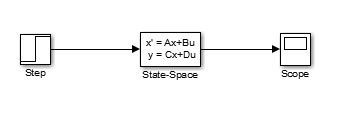
\includegraphics[width=\textwidth]{slinear.PNG}
    \caption{Schéma SimuLink modèles Linéaire }
    \label{fig:Part1}
\end{figure}

Pour le modèle linéaire, nous le soummetons à une entrée nulle avec une condition initiale égale à $-X_0$. Nous obtenons en sortie, un signal qui converge vers $0$ <<Figure:\ref{fig:linéar}>> et qui représente le point d'équilibre du modèle linéaire.  


\begin{figure}[H]
    \centering
    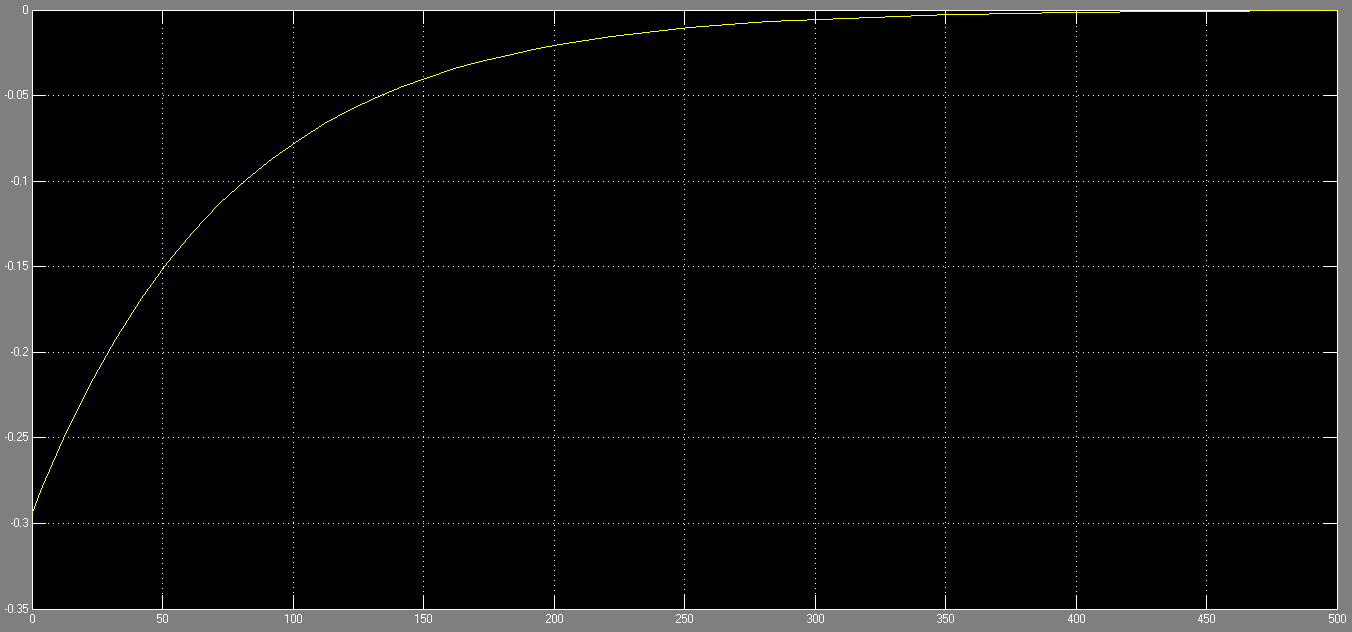
\includegraphics[width=\textwidth]{linear.PNG}
    \caption{Résultats du modèle linéarisé }
    \label{fig:linéar}
\end{figure}


\begin{figure}[H]
    \centering
    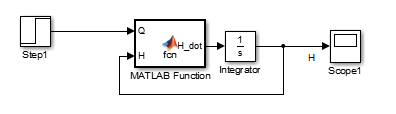
\includegraphics[width=\textwidth]{snonlinear.PNG}
    \caption{Schéma SimuLink du modèle Non-linéaire }
    \label{fig:snonlinéar}
\end{figure}

la réponse du modèle non-linéaire pour une condition initiale égale à $0$ est représentée par la figure \ref{fig:nonlinéar}, qui converge convèrge vers le point d'équilibre $X_0$ comme prédit théoriquement.



\begin{figure}[H]
    \centering
    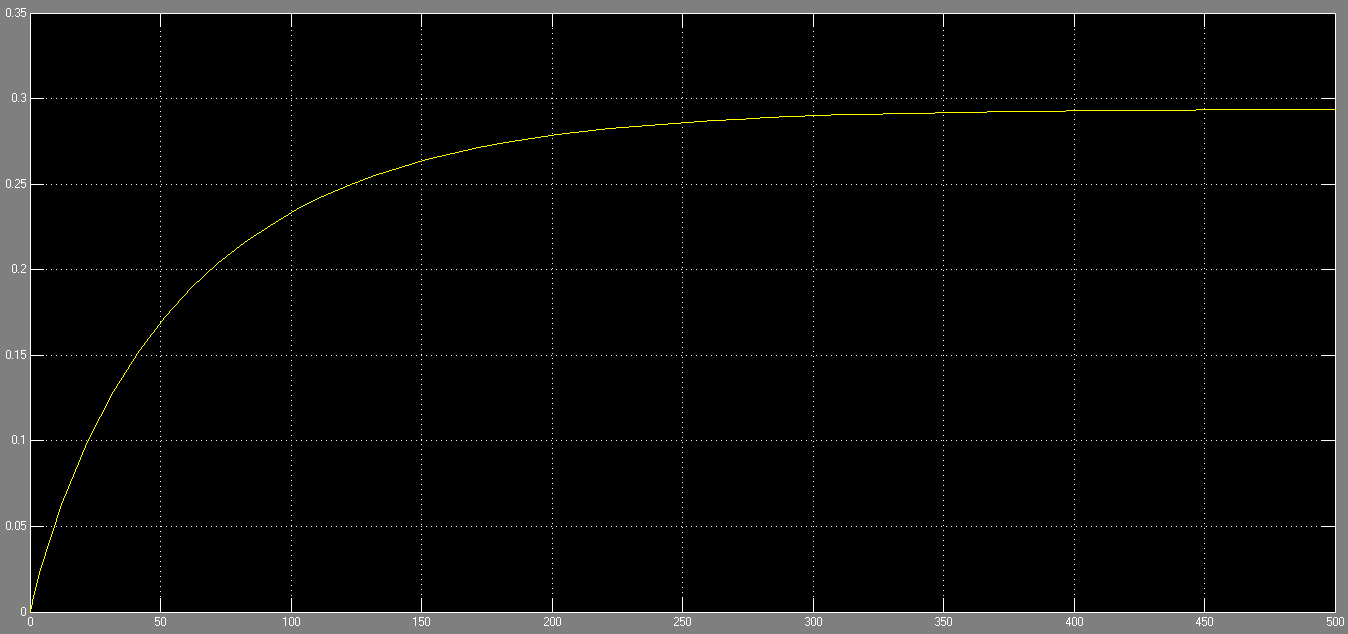
\includegraphics[width=\textwidth]{nonlinear.PNG}
    \caption{Résultats du modèle non-linéare }
    \label{fig:nonlinéar}
\end{figure}     


\section{\textsc{Fonction de Lyapunov pour le modèle linéaire}}

	\paragraph{}
	La fonction: $V(\delta_x)=\frac{\delta_x^2}{2}$ qui est définie positive pour $\forall \delta_x \in R $ et qui est de classe $C1$, correspondra à notre fonction de Lyapunov choisie pour notre cas.\\

	\par	 La dérivée de cette fonction est de cette forme: 
	\begin{center}
		$\dot{V}(\delta_x) = \frac{dV(\delta_x)}{dt} = \frac{dV(\delta_x)}{d\delta_x} \frac{d\delta_x}{dt} = \frac{dV(\delta_x)}{d\delta_x} \dot{\delta_x} $\\[0.25 cm]
		$ \dot{V}(\delta_x) = \delta_x \dot{\delta_x} = \frac{-S_n}{S} \sqrt{\frac{g}{2X_0}} \delta_x^2 $\\[0.25 cm]
		%$ \dot{V}(x) = \frac{-S_n}{S} \sqrt{\frac{g}{2X_0}} x^2 + \frac{u}{S} x $
	\end{center} 
	\par Cette dérivée,$\dot{V}(\delta_x)$ est définie négative $\dot{V}(\delta_x)<0 \hspace{1mm} \forall \delta_x \in R $. Alors on pourra conclure que le système étudié est localement asymptotiquement stable.
	
\break
\section{\textsc{Fonction de Lyapunov pour le modèle non-linéaire}}
		
		\par On sait que  $\dot{V}(\delta_x) = \delta_x \dot{\delta_x} $, alors:\\

		Rappel: $ \dot{x}=\frac{1}{S_n} u - \frac{S_n}{s} \sqrt{2 g x}$, avec:
		\begin{center}
		 $ x = H(t)$ \\[0.25 cm]
		 $ X_0 = \frac{1}{2g} \frac{Q^2_0}{S^2_n}$ \\[0.25 cm]
		 $ \delta_x = H(t)-X_0 = x-X_0 $ \\[0.25 cm]
		 $ u = Q(t) = Q_0 $
		\end{center}
		
		En faisant un changement de variable de $ \dot{V}(\delta_x) $ vers $ \dot{V}(x) $ la fonction dérivée de Lyapunov devient:
		\begin{center}
			
		 $\dot{V}(x) = (x - X_0 ) ( \frac{1}{S} u - \frac{S_n}{s} \sqrt{2 g x}) $\\[0.25 cm]		
		
		 $\dot{V}(x) = (x - \frac{1}{2g} \frac{Q^2_0}{S^2_n} ) ( \frac{1}{S} Q_0 - \frac{S_n}{s} \sqrt{2 g x}) $\\[0.25 cm]
		 $ \dot{V}(x) = \frac{1}{2g} (2g x - \frac{Q^2_0}{S^2_n} ) \frac{S_n}{s}( \frac{1}{S_n} Q_0 - \sqrt{2 g x})$ \\[0.25 cm]
		 $ \dot{V}(x) =\frac{-S_n}{2gs}(2g x - \frac{Q^2_0}{S^2_n} ) ( \sqrt{2gx} - \frac{Q_0}{S_n} ) $
		 \end{center}
		 
	\par La quantité $ ( \sqrt{2gx} - \frac{Q_0}{S_n} ) > 0 \forall x  $ donc la quantité $ (2g x - \frac{Q^2_0}{S^2_n} ) $ l'est aussi $\forall x$, ça implique que $ \dot{V}(x) $ est définie négative pour $\forall x$. De cette manière la fonction de Lyapunov de base utilisée pour le système linéarisé est aussi une fonction de Lyapunov pour le modèle non-linéaire avec entrée $Q_0$.
	  		 
%\chapter{\textsc{Analyse du procédé de deux bacs d'eau sans entrée}}
\section{\textsc{Le procédé}}
 
 \paragraph{} Le système représenté sur la Figure 2 est composé de deux bacs cylindriques de section $S$. Ils sont reliés par
un tuyau de section $S_n << S$, où l’eau peut circuler dans les deux directions. Lors de cette manipulation, nous
allons nous intéresser au niveau de l’eau $H_1 (t)$ et $H_2 (t)$.

\paragraph{} Les valeurs données par le constructeur sont : $ S = 0.0154m^2 $ et $S_n = 5 \times 10^{-5}m^2 $. Les valeurs initiales sont $ H_1 (0) = 0.3m $ et $ H_2 (0) = 0.2m $.

	\begin{center}
	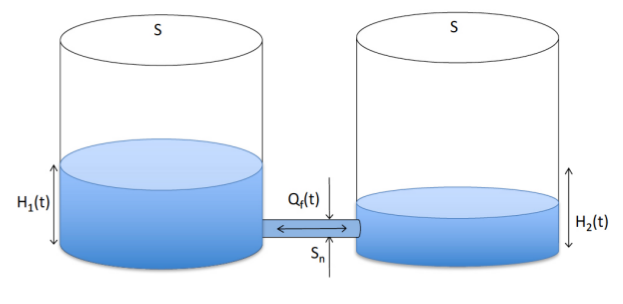
\includegraphics[scale=0.5]{2bac.png}
	\captionof{figure}{\textit{Deux bacs d'eau sans source et fuite\\}}
	\label{fig2} 
	\end{center}
	
\section{\textsc{Modélisation du système par un bilan de volume}}

	Nous avons:
\begin{center}
    $$\left\{
\begin{array}{l}
    V(t)=S\times H(t)\\
    \dot{V}(t)=S\times \dot{H}(t)=(Q(t)-Q_f(t)) ;\text{ avec Q(t) = $0$.}\\
    Q_f(t)=S_n \times V_n \ ; \ \ \ avec\indent  V^2_n = 2\times g\times |H_1(t)-H_2(t)| 

\end{array}
\right.$$
\end{center}


Donc $Q_f(t)=S_n\sqrt{2g |H_1(t)-H_2(t)|}$\\\\
On pose:  $ x= H_1 - H_2$

\[\Longrightarrow Q_f=S_n\times \sqrt{2\times g \times |x|}\]
\[\Longrightarrow \dot{x}=-\frac{Q_f}{S}=-sign(x)\times \frac{S_n\times \sqrt{2\times g }}{S} \times \sqrt{|x|}\]
\[\color{red}\dot{x}=-sign(x)\times \frac{S_n\times \sqrt{2\times g }}{S} \times \sqrt{|x|}\]
 Avec: \textbf{sign(x)} représente le sens de l'écoulement de l'eau entre les deux bacs. \\
 
\textbf{Hypothèse:} on suppose que $H_1>H_2$.\\
\\
Alors:\indent \indent  \[\dot{x}= -\frac{S_n\times \sqrt{2\times g }}{S} \times \sqrt{x}\]
\\
\\
\\\\\\\\

\section{Détermination du point d'équilibre}

On cherche \textbf{x} tel que \textbf{x}= Cst = $\textbf{X}_0$

\[0=-\frac{S_n\times \sqrt{2\times g }}{S} \times \sqrt{X_0}\indent  \Longrightarrow \indent X_0 = 0\]
Cela signifie que le niveau de l'eau dans les deux bacs est le même $H_1=H_2$.

\section{Linéarisation autour du point d'équilibre:}

\[\dot{\delta_x}=f(X_0+\delta_x) \indent \Longrightarrow \indent \dot{\delta_x}=f(X_0)+\frac{\partial f}{\partial x}(X_0).\delta(x)\]
Sachant que $f(X_0)=0$ ;\indent  $\Longrightarrow \indent \dot{\delta_x}=\frac{\partial f}{\partial x}_{|X_0} . \delta_x$
\[\dot{\delta_x}=\begin{bmatrix}\frac{-S_n\times \sqrt{2\times g}}{2\times S \times \sqrt{X0}}\end{bmatrix}.\delta_x \ \ ; \indent \longleftarrow \indent \text{Or, ceci est impossible}\]
Donc, la linéarisation est impossible.	
	
\section{\textsc{Fonction de Lyapunov pour le modèle non-linéaire}}

	\par On choisira la même fonction utilisée précédemment soit :$ V(x) \frac{x^2}{2} $, sa dérivée devient:
	 
	\begin{center}
	
		$ \dot{V} (x) = \frac{-S_n}{S} \sqrt{2gx} \hspace{1mm} x  \hspace {0.5 cm} $ si $H_1(t) > H_2(t) $	
	 
	\end{center}
	\par Sachant que $x=H_1(t) - H_2(t)$ alors $x>0$ or la quantité $\frac{-S_n}{S} \sqrt{2gx}<0$, cela prouve que $\dot{V}(x)$ est définie négative pour $H_1(t) > H_2(t)$, le deuxième cas présente:  
	
	\begin{center}
	
		$ \dot{V} (x) = \frac{S_n}{S} \sqrt{2gx}\hspace{1mm} x \hspace{0.5 cm}$ si $H_1(t) < H_2(t) $
			
	\end{center}
	
	\par Sachant que dans ce cas $x<0$ et la quantité $\frac{S_n}{S} \sqrt{2gx}>0$ alors $V(x)$ est définie négative si $H_1(t) < H_2(t)$
	\par De cette façon la fonction dérivée de Lyapunov est définie négative pour les deux cas, donc le système est globalement asymptotiquement stable. 
	 
%\input{chap4&5.tex}
%\input{conclusion.tex}
%\input{annexes.tex}
%*********************** Bibliographie ************ 
\bibliographystyle{alpha}
\bibliography{biblio}  



\end{document}